\section{Device Specifications}

\subsection{Sensor Board: CM5000}

\begin{figure}[H]
\centering
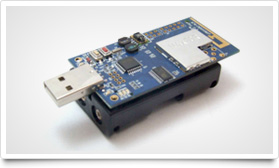
\includegraphics[scale=0.5]{Images/CM5000}
\end{figure}

\begin{table}[H]
	\centering
	\begin{tabular}{| l | l | p{5.5cm} |}
	\hline
	\textbf{Item} & \textbf{Specification} & \textbf{Description} \\
	\hline
	\hline

	\multicolumn{3}{|l|}{\textbf{Processor}} \\
	\hline
	Processor Model & Texas Instruments\textregistered~ MSP430F1611 & Texas Instruments\textregistered~ MSP430 family\\
	\hline
	\multirow{3}{*}{Memory} & 48KB & Program Flash \\
	~ & 10KB & Data RAM \\
	~ & 1MB & External Flash (ST\textregistered~ M25P80) \\
	\hline
	ADC & 12bit resolution & 8 channels \\
	\hline
	\multirow{2}{*}{Interfaces} & UART, SPI, I2C & Serial Interfaces \\
	~ & USB & External System Interface (FTI\textregistered~ FT232BM) \\
	\hline
	\hline

	\multicolumn{3}{|l|}{\textbf{Radio}} \\
	\hline
	RF Chip & Texas Instruments\textregistered~ CC2420 & IEEE 802.15.4 2.4GHz Wireless Module\\
	\hline
	Frequency Band & 2.4GHz \mytilde 2.485GHz & IEEE 802.15.4 compliant \\
	\hline
	Sensitivity & -95dBm typ & Receive Sensitivity \\
	\hline
	Transfer Rate & 250Kbps & IEEE 802.15.4 compliant \\
	\hline
	RF Power & -25dBm \mytilde 0dBm & Software Configurable \\
	\hline
	Range & \mytilde120m (outdoor), 20\mytilde30m (indoor) & Longer ranges possible with optional SMA antenna attached \\
	\hline
	\multirow{3}{*}{Current Draw} & RX: 18.8mA & \multirow{3}{5.5cm}{Lower RF Power Modes reduce consumption} \\
	~ & TX: 17.4mA & ~ \\
	~ & Sleep mode: 1uA & ~ \\
	\hline
	RF Power Supply & 2.1V \mytilde 3.6V & CC2420 Input Power \\
	\hline
	Antenna & Dipole Antenna / PCB Antenna & Additional SMA connector available for extra antenna \\
	\hline
	\hline

	\multicolumn{3}{|l|}{\textbf{Sensors}} \\
	\hline
	Light 1 & Hamamatsu® S1087 Series & Visible Range (560 nm peak sensitivity wavelength)\\
	\hline
	Light 2 & Hamamatsu® S1087 Series & Visible \& Infrared Range (960 nm peak sensitivity wavelength)\\
	\hline
	\multirow{6}{2.5cm}{Temperature \& Humidity} &  \multirow{6}{*}{Sensirion® SHT11} & Temperature Range: -40 \mytilde 123.8 $^\circ$C  \\
	~ & ~ & Temperature Resolution: $\pm$ 0.01 (typical) \\
	~ & ~ & Temperature Accuracy: $\pm$ 0.4 $^\circ$C (typical) \\
	~ & ~ & Humidity Range: 0 \mytilde 100\% RH \\
	~ & ~ & Humidity Resolution: 0.05 (typical) \\
	~ & ~ & Humidity Accuracy: $\pm$ 3 \%RH (typical) \\
	\hline

	\end{tabular}
	\caption{Specifications for the CM5000 Wireless Sensor Node \cite{CM5000}}
	\label{tab:CM5000-spec}
\end{table}

\clearpage


\subsection{Interface Module: USB1000}

\begin{figure}[H]
\centering
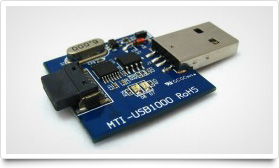
\includegraphics[scale=0.5]{Images/USB1000}
\end{figure}

\begin{table}[H]
	\centering
	\begin{tabular}{| l | l | p{5.5cm} |}
	\hline
	\textbf{Item} & \textbf{Specification} & \textbf{Description} \\
	\hline
	\hline

	\multicolumn{3}{|l|}{\textbf{Components}} \\
	\hline
	Interface Type & USB type A & USB 1.1 compatible. USB full speed support (12Mbps)\\
	\hline
	USB2UART Chip & FTDI\textregistered~ FT232BM & USB2UART converter chip\\
	\hline
	1kbit EEPROM & Microchip® 93C46 & Driver ID storage\\
	\hline
	Quad Buffer & Texas Instruments\textregistered~ SN74HC126 & USB Rx/Tx Communications buffer\\
	\hline
	Octal Switch & Analog Devices\textregistered ADG715 & Reset sequence recognition\\
	\hline
	Mote Interface & Terminal Block (ERNI\textregistered~ compatible) & Connector to CMXX00 WSN Motes (Vcc, GND, 8 port ADC, 2 port GPIO pins)\\
	\hline

	\end{tabular}
	\caption{Specifications for the USB1000 Interface Board \cite{USB1000}}
	\label{tab:USB1000-spec}
\end{table}

\clearpage

\subsection{Network Infrastructure: UD1000}

\begin{figure}[H]
\centering
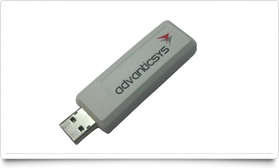
\includegraphics[scale=0.5]{Images/UD1000}
\end{figure}

\begin{table}[H]
	\centering
	\begin{tabular}{| l | l | p{4.5cm} |}
	\hline
	\textbf{Item} & \textbf{Specification} & \textbf{Description} \\
	\hline
	\hline

	\multicolumn{3}{|l|}{\textbf{Processor}} \\
	\hline
	Processor Model & Texas Instruments\textregistered~ MSP430F1611 & Texas Instruments\textregistered~ MSP430 family\\
	\hline
	\multirow{2}{*}{Memory} & 48KB & Program Flash \\
	~ & 10KB & Data RAM \\
	\hline
	ADC & 12bit resolution & 8 channels \\
	\hline
	\multirow{2}{*}{Interfaces} & UART, SPI, I2C & Serial Interfaces \\
	~ & USB & External System Interface (FTI\textregistered~ FT232BM) \\
	\hline
	\hline

	\multicolumn{3}{|l|}{\textbf{Radio}} \\
	\hline
	RF Chip & Texas Instruments\textregistered~ CC2420 & IEEE 802.15.4 2.4GHz Wireless Module\\
	\hline
	 Frequency Band & 2.4GHz \mytilde 2.485GHz & IEEE 802.15.4 compliant \\
	\hline
	Sensitivity & -95dBm typ & Receive Sensitivity \\
	\hline
	Transfer Rate & 250Kbps & IEEE 802.15.4 compliant \\
	\hline
	RF Power & -25dBm \mytilde 0dBm & Software Configurable \\
	\hline
	Range & \mytilde40m (outdoor), 15\mytilde20m (indoor) & Dongle orientation dependent \\
	\hline
	\multirow{3}{*}{Current Draw} & RX: 18.8mA & \multirow{3}{4.5cm}{Lower RF Power Modes reduce consumption} \\
	~ & TX: 17.4mA & ~ \\
	~ & Sleep mode: 1uA & ~ \\
	\hline
	RF Power Supply & 2.1V \mytilde 3.6V & CC2420 Input Power \\
	\hline
	Antenna & Ceramic antenna & ~ \\
	\hline
	\hline

	\multicolumn{3}{|l|}{\textbf{Electromechanical Characteristics}} \\
	\hline
	Dimensions & 65mm x 22.5mm x 14mm & Including housing\\
	\hline
	Weight & 15g & ~\\
	\hline
	Power & 5V  & DC over USB\\
	\hline
	Current & 90mA  & Max rated current over USB\\
	\hline
	Operating Temperature & -25$^\circ$C \mytilde +60$^\circ$C & ~\\
	\hline
	Storage Temperature & -40$^\circ$C \mytilde +60$^\circ$C & ~\\
	\hline
	Operating Humidity & 5\% \mytilde 95\% & Non condensing\\
	\hline
	Protection type & IP20 & Non condensing\\
	\hline

	\end{tabular}
	\caption{Specifications for the UD1000 Sensor Network Sink \cite{UD1000}}
	\label{tab:UD1000-spec}
\end{table}
